\documentclass[11pt, a4paper, twoside]{article}   	% use "amsart" instead of "article" for AMSLaTeX format

\usepackage{geometry}                		% See geometry.pdf to learn the layout options. There are lots.
\usepackage{pdfpages}
\usepackage{caption}
\usepackage{minted}
\usepackage[german]{babel}			% this end the next are needed for german umlaute
\usepackage[utf8]{inputenc}
\usepackage{color}
\usepackage{graphicx}
\usepackage{titlesec}
\usepackage{fancyhdr}
\usepackage{lastpage}
\usepackage{hyperref}
\usepackage[autostyle=false, style=english]{csquotes}
\usepackage{mathtools}
\usepackage{tabularx}
% http://www.artofproblemsolving.com/wiki/index.php/LaTeX:Symbols#Operators
% =============================================
% Layout & Colors
% =============================================
\geometry{
   a4paper,
   total={210mm,297mm},
   left=20mm,
   right=20mm,
   top=20mm,
   bottom=30mm
 }	

\definecolor{myred}{rgb}{0.8,0,0}
\definecolor{mygreen}{rgb}{0,0.6,0}
\definecolor{mygray}{rgb}{0.5,0.5,0.5}
\definecolor{mymauve}{rgb}{0.58,0,0.82}

\setcounter{secnumdepth}{4}


% the default java directory structure and the main packages
\newcommand{\srcDir}{../src/}
\newcommand{\imageDir}{./images/}
% =============================================
% Code Settings
% =============================================
\newenvironment{code}{\captionsetup{type=listing}}{}
\newmintedfile[mSourceFile]{matlab}{
	linenos=true, 
	frame=single, 
	breaklines=true, 
	tabsize=2,
	numbersep=5pt,
	xleftmargin=10pt,
	baselinestretch=1,
	fontsize=\footnotesize
}
\newmintinline[mInlineSource]{matlab}{}
\newminted[mSource]{matlab}{
	breaklines=true, 
	tabsize=2,
	autogobble=true,
	breakautoindent=false
}
% =============================================
% Page Style, Footers & Headers, Title
% =============================================
\title{Übung 1}
\author{Thomas Herzog}

\lhead{Data Warehouse}
\chead{}
\rhead{
\includegraphics[scale=0.10]{FHO_Logo_Students.jpg}}

\lfoot{S1610454013}
\cfoot{}
\rfoot{ \thepage / \pageref{LastPage} }
\renewcommand{\footrulewidth}{0.4pt}
% =============================================
% D O C U M E N T     C O N T E N T
% =============================================
% =============================================
% 2016.10.13: 1 
% 2016.10.14: 2
% =============================================

\pagestyle{fancy}
\begin{document}
\setlength{\headheight}{15mm}
%\includepdf[pages={1,2}]{Uebungszettel02.pdf}

\section{Data import and preparation}
This part of the document deals with the data preparation of the provided cooper wire data before the data analysis.

\subsection{Data import}

\begin{figure}[h]
\centering
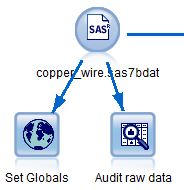
\includegraphics[scale=1]{\imageDir/dm-spss-import-data.JPG}
\caption{Data import in Stream}
\end{figure}
\ \newline
The data is imported via the node \emph{SAS file}. The node \emph{Set Globals} is used for setting the audited data results of the raw imported data as global values, which get used later on for the data preparation. The node \emph{Data Audit} is used for analyzing the raw data.

\begin{figure}[h]
\centering
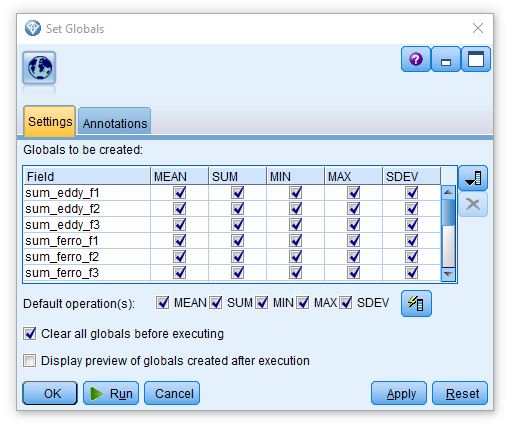
\includegraphics[scale=1]{\imageDir/dm-spss-set-globals.JPG}
\caption{Set audit results as global values in the stream}
\end{figure}
\subsection{Data preparation}
The outliers and extremes where determined during the audit of the raw data.
\begin{figure}[h]
\centering
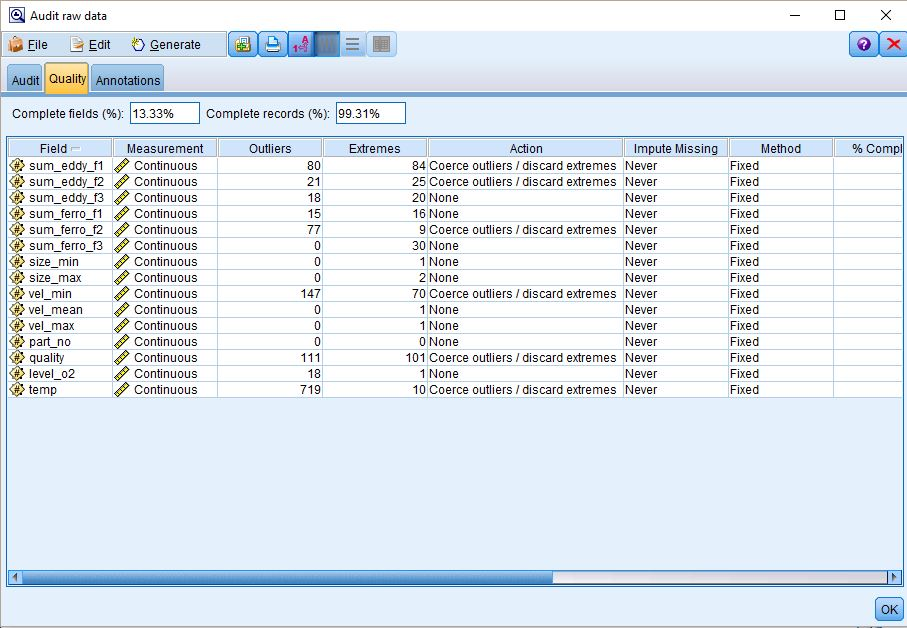
\includegraphics[scale=0.6]{\imageDir/dm-spss-raw-audit.JPG}
\caption{Audit of the raw data}
\label{fig:raw-data-audit}
\end{figure}
\begin{figure}[h]
\centering
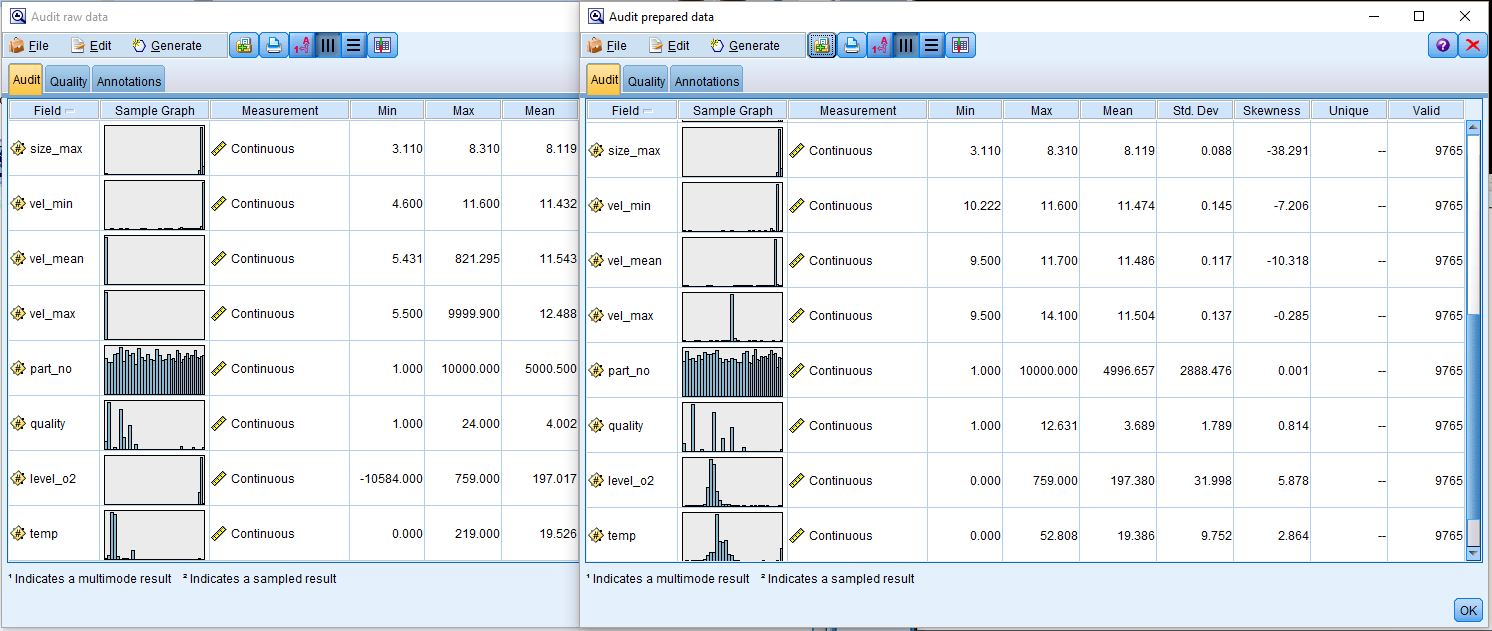
\includegraphics[scale=0.4]{\imageDir/dm-spss-audit-prepared-data.JPG}
\caption{Audit of the raw data}
\end{figure}
\ \newpage

\begin{figure}[h]
\centering
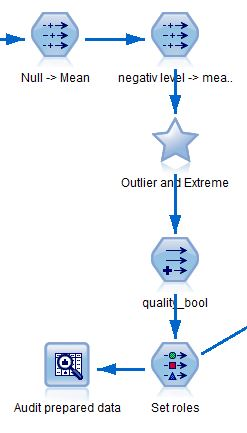
\includegraphics[scale=1]{\imageDir/dm-spss-data-preparation-flow.JPG}
\caption{Flow of data preparation tasks}
\end{figure}
\ \newline
This flow prepares the data for the later analysis. The following tasks are performed:
\begin{itemize}
	\item Null values will be replaced with the mean value set by the \emph{Set Global} node
	\item The negative value of the field \emph{temp} will be replaced with the global mean of this field
	\item The outliers and extremes will be handled as you can see in image \ref{fig:raw-data-audit}
	\item A new filed will be created \emph{quality\_bool} which represents the quality state good or false
	\item The fields which are not considered to be relevant will be set as ignored and the field \emph{quality\_bool} will be set as the target field for the further analysis
\end{itemize}
\ \newpage

\subsection{Predictive Model}
\begin{figure}[h]
\centering
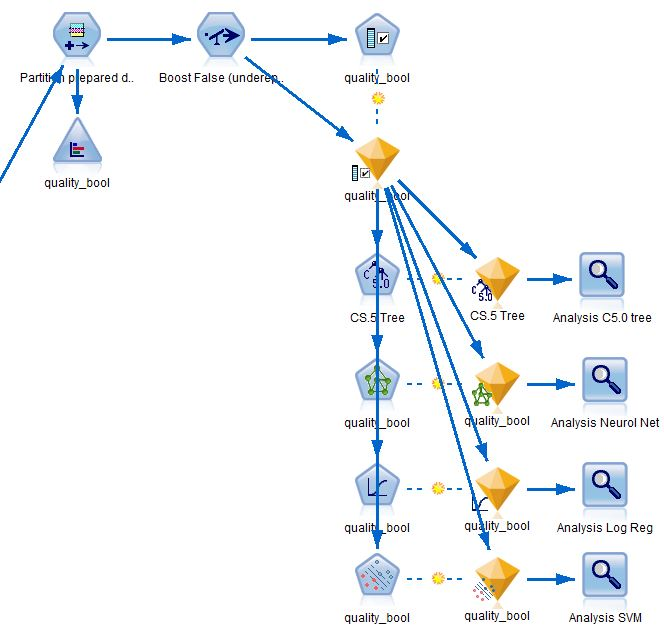
\includegraphics[scale=0.7]{\imageDir/dm-spss-predictive-model.JPG}
\caption{Flow of the predictive model}
\end{figure}
\ \newline
The flow of the predictive part of the model uses the following nodes:
\begin{itemize}
	\item \emph{C5.0} (The decision tree)
	\item \emph{Neural Net}
    \item \emph{Logistic} (Logistic Regression)
    \item \emph{SVM}
\end{itemize}
\ \newline
Each modeling node gets analyzed with the node \emph{Analyze}.
\newpage

\subsection{Fine tuning}


\end{document}
